% テクニカルレポート（日本語版、下書き）。ビルド: bash docs/report/build.sh
\documentclass[10pt,a4paper,twocolumn]{article}
\usepackage[margin=17mm,columnsep=6mm]{geometry}
\usepackage{amsmath,amssymb}
\usepackage{booktabs}
\usepackage{graphicx}
\usepackage{xcolor}
\usepackage{tikz}
\usetikzlibrary{positioning,arrows.meta,fit,calc}
\usepackage[font=small,labelfont=bf,labelsep=quad]{caption}
\usepackage{enumitem}
\setlist{nosep,leftmargin=*}
\usepackage{xeCJK}
\setCJKmainfont[Path=fonts/,BoldFont=NotoSerifJP-Bold.otf]{NotoSerifJP-Regular.otf}
\setCJKsansfont[Path=fonts/,BoldFont=NotoSansJP-Bold.otf]{NotoSansJP-Regular.otf}
\usepackage[colorlinks=true,linkcolor=blue!50!black,citecolor=blue!50!black,urlcolor=blue!50!black]{hyperref}
\renewcommand{\abstractname}{概要}
\renewcommand{\refname}{参考文献}
\renewcommand{\figurename}{図}
\renewcommand{\tablename}{表}
\newcommand{\pt}{\,pt}
\setlength{\emergencystretch}{1.5em}
\linespread{1.03}

\title{\Large\bfseries 声の物理モデルをデコーダにした音声コーデック:\\
制御列を書くエンコーダと、制御列の上の音声合成}
\author{Claude（Anthropic）\thanks{Claude（Fable 5.2）が Claude Code 上で、実験の計画と実装、実行、
結果の分析、本稿の執筆を行った。森 琢磨は、試聴とおおまかなディレクションを行った。}\qquad 森 琢磨}
\date{{\small テクニカルレポート（下書き）、2026 年 11 月}\\
{\small\url{https://github.com/takuma104/physical-modeling-voice-codec}}}

\begin{document}
\maketitle

\begin{abstract}
ニューラル音声コーデックは、どんな潜在表現も音に変える。潜在表現を予測するモデルが誤ると、声道では
出せない音が出ることがある。本稿では、それができないデコーダを持つコーデックを調べる。デコーダは、
人の声の物理モデル CHIMERA（肺、声帯、枝分かれした声道。オープンソース）で、改造せずに使う。
潜在表現はその制御列で、100\,Hz・21 チャネルである。顎、舌、唇、軟口蓋の位置と、声門の状態、
息、声の高さを表す。エンコーダは、録音からこの制御列を 1 回の推論で書く。学習には文の書き起こしも
制御列の探索も使わない。シミュレータは微分できないので、その代役となるネットワークを通して教える。
学習に使っていない英語の話者で、合成音を Whisper が読み誤る単語は 3.2\%（実録音は 1.6\%）、
日本語では音素の 0.4\%（同 0.2\%）である。制御列へのノイズ、4 bit の量子化、25\,Hz への間引きでは
音声は少しずつ崩れ、耳には滑舌の悪い人の誤りに聞こえる。実録音にない 2 種類の音を、試聴を手がかりに
シミュレータ自身の仕組みまでたどり、公開されている設定で取り除いた。音素から制御列を書く音声合成
モデルは、エンコーダと同じだけ聞き取れる（0.2\% 対 0.1\%）。1 話者の 200 文（15 分）で学習すると
音素の誤りは 0.5\%、20 文（1.5 分）でも 7.7\% である。このうち何が潜在表現のおかげかを、対照実験で
確かめた。同じモデルにメルスペクトログラムや EnCodec の潜在表現を書かせても、同じ少ないデータで
同じだけ聞き取れる。これはモデルの性質である。デコーダの違いは、データが少ないときの音に出る。
20 文と 200 文で、物理モデルの予測品質は 4.1 と 4.8、メルスペクトログラムは 2.6 と 3.5 で、モデルの
出力でボコーダを調整しても 3.2 と 4.1 までである。2,000 文あれば、調整したボコーダは実録音と同じ
4.5 に届く。100 話者で学習すると、見たことのない文を実録音と同じだけ聞き取れる音で
読む（2.3\% 対 2.5\%）。話者についてコーデックが運ぶのは、性別と声の高さである。シミュレータの
体格・声門・構えの癖を話者ごとに当てはめる（値を 11 個足す）と、話者照合モデルが 8 話者の中から
本人を選ぶ割合が 26.5\% から 57.0\% に、100 話者の中からでは 2.8\% から
14.2\% に上がる（実録音は 96.5\% と 93.7\%）。
\end{abstract}

\section{はじめに}
ニューラル音声コーデック~\cite{encodec,moshi} は、現在の音声生成の接点になっている。言語モデルや
フローモデルが潜在表現を予測し、ニューラルデコーダが波形に変える。デコーダはどんな潜在表現でも
受け取る。予測するモデルが小さいか、データが少ないと、その誤りは「分布から外れた潜在表現を
デコーダがどう鳴らすか」として現れる。うなり、金属的な子音、口の中に音源のない音である。著者の
1 人は、Mimi コーデックの上に作られた Pocket TTS を日本語に対応させる中でこれに出会った~\cite{pocketja}。

本稿は、デコーダを声の物理モデルにしたらどうなるかを調べる。声帯と声道を通る空気の流れの
シミュレータは、そういう系が出せる音しか出せない。その制御パラメータを潜在表現にすれば、潜在表現の
誤りは、舌の位置のずれや声門の閉じ遅れになる。つまり調音の誤りで、人の誤り方と同じである。仮説は、
そういうコーデックは崩れ方が穏やかであり、また、その潜在表現は音声を作っているものに近いので、
テキストから予測しやすい、というものである。

調音を介した音声符号化には長い歴史がある。近年のニューラルな研究は、音声を調音の軌跡に符号化し、
ニューラルボコーダで復号する。SPARC~\cite{sparc}（調音器官の 12 座標と声の高さ、音量を 50\,Hz で。
デコーダは HiFi-GAN）や ARTI-6~\cite{arti6}（リアルタイム MRI から得た 6 特徴）である。これらの
デコーダはネットワークのままである。声道の微分可能なシミュレーション~\cite{difftlm} は、発話ごとの
最適化で音声から声道の形を復元する。VocalTractLab~\cite{vtl} のような調音合成器は、規則か、
合成による分析で駆動される。

本稿では、物理合成器 CHIMERA~\cite{chimera} をそのまま使い、残りをその周りに作る。
\begin{itemize}
\item 録音からシミュレータの制御列を 1 回の推論で書く\textbf{エンコーダ}。書き起こしを使わず、
シミュレータの代役を学習して、それを通して教える（\ref{sec:encoder} 節）。
\item \textbf{潜在表現の誤りが人の声のままである}ことの確認。制御列へのノイズ、量子化、間引き
（\ref{sec:perturb} 節）。
\item 試聴で見つけた\textbf{シミュレータ由来の 2 種類の音}を、仕組みまでたどって設定で取り除く
こと、および高い声のための設定（\ref{sec:voice} 節）。
\item 潜在表現の上の\textbf{音声合成モデル}。エンコーダと同じだけ聞き取れ、数分の音声から
学習できる（\ref{sec:tts} 節）。
\item \textbf{対照実験}。同じモデルに 3 種類のニューラルデコーダの潜在表現を書かせ、物理デコーダが
何に効いていて、何に効いていないかを確かめる（\ref{sec:control} 節）。
\end{itemize}
コードは上記のリポジトリにある。エンジンのコードは一切変更していない。

\section{デコーダと潜在表現}\label{sec:decoder}
\textbf{CHIMERA}~\cite{chimera} は、Rust で書かれた物理モデルの音声合成器（MIT ライセンス）で、
ブラウザで鳴らす楽器として作られている。気道を時間領域で、48\,kHz でシミュレートする。肺の圧力、
声帯（その面積の波形が声門の開口を動かし、流量は前後の圧力差から決まるので、パルスの歪みや、口を
閉じたときの無声化は物理から出てくる）、鼻腔と側面の通路を持つ枝分かれした声道、唇・鼻・壁からの
放射、そして流れが狭め・歯・声門を通るところの帯域制限された雑音である。\emph{体格}のパラメータが、
男性・女性・子どもの声道の大きさを連続的に混ぜる。付属のフロントエンドは、英語のテキストを規則で
ジェスチャに変える。

\textbf{制御列。}フロントエンドは使わない。小さなラッパー（PyO3）が、10\,ms ごとに 21 個の制御値の
フレームを、エンジンの調音器官と音源の目標値として予約する（図~\ref{fig:channels}）。制御列のほかに
声に伝える話者の情報は 2 つだけである。体格を選ぶ性別と、声の高さの中央値である。それ以上の
話者性は、潜在表現に含まれない（\ref{sec:discussion} 節）。

\begin{figure}[t]
\centering
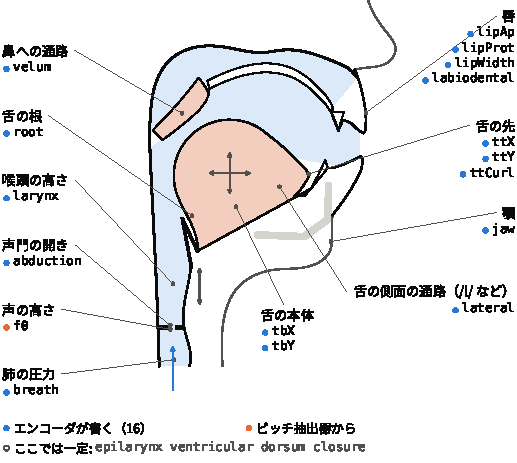
\includegraphics[width=\columnwidth]{fig_tract_ja.pdf}
\caption{デコーダの声道と、制御列の 21 チャネル（100\,Hz）。輪郭は CHIMERA 自身のもので、男性の体格で
口を半分開いた母音、鼻への通路は開いた姿勢である。シミュレートするのは、輪郭の間の空気（青）である。
各チャネルは、調音器官 1 つ、または音源の目標値である。エンコーダは発話の中で動く 16 個を書く。
声の高さはピッチ抽出器から取る。4 個は一定にしておく。}
\label{fig:channels}
\end{figure}

\textbf{制御列で足りるか。}CHIMERA の規則による合成音を、その制御列（100\,Hz）から鳴らし直しても、
ほとんど変わらない。元の音とのメルケプストラム距離は 0.7\,dB で、有声・無声は 97\% のフレームで
一致する。CPU の 1 スレッドで、4 秒の文を 0.5 秒で鳴らせる。

\textbf{データと物差し。}英語は TSP speech database~\cite{tsp}（無響室で読まれた Harvard sentences）
で、4 話者（240 録音）をテストに、2 話者を検証に、その話者が読む文リストごと取り置き、1,012 録音が
残る。日本語は JVS~\cite{jvs}（100 話者）、Hi-Fi-CAPTAIN~\cite{hificaptain}（女性 1 人、男性 1 人）、
JSUT~\cite{jsut} である。結果はすべて、本稿のどの学習も調整も最適化の対象にしていないモデルで測る。
Whisper~\cite{whisper} の small（英語は small.en）と large-v3-turbo を貪欲復号で使い、英語は単語、
日本語は Open JTalk~\cite{openjtalk} の読みの音素で数える。もう 1 つは、テキストを知らない多言語の
音声記号認識器~\cite{xlsrphone} で、録音と合成音を国際音声記号で書き取らせる（\emph{音声記号の
不一致}: 録音側の記号のうち合成音側で変わった割合。同じ文を別の人が読んだ録音は、日本語で
24--32\% になる）。予測品質は NISQA~\cite{nisqa} で、設定を選ぶのに 2 か所で使い（\ref{sec:voice} 節、
\ref{sec:control} 節）、数値はそれに使っていない録音のものを載せる。これは NISQA の音声品質の
モデルである。合成音声の自然さを予測するモデルもあり、そちらはシミュレータの声を低く付ける
（\ref{sec:control} 節で報告する）。

\section{エンコーダ}\label{sec:encoder}
\begin{figure}[t]
\centering\footnotesize
\begin{tikzpicture}[
  box/.style={draw, rounded corners=2pt, minimum height=6mm, inner xsep=2pt, align=center, font=\scriptsize},
  phys/.style={box, fill=black!8},
  arr/.style={-{Stealth[length=1.6mm]}, semithick},
  learn/.style={-{Stealth[length=1.6mm]}, semithick, densely dashed}]
\node[box] (rec) {録音};
\node[box, right=3.5mm of rec] (enc) {エンコーダ};
\node[box, right=3.5mm of enc, fill=blue!8] (trk) {制御列\\21\,ch $\times$ 100\,Hz};
\node[phys, right=3.5mm of trk] (sim) {CHIMERA\\（無改造）};
\node[box, below=7mm of enc] (tts) {TTS モデル};
\node[box, left=3.5mm of tts] (txt) {音素、\\アクセント};
\node[box, below=7mm of sim] (std) {声の代役};
\node[box, above=7mm of trk] (lis) {リスナーの特徴};
\draw[arr] (rec) -- (enc); \draw[arr] (enc) -- (trk); \draw[arr] (trk) -- (sim);
\draw[arr] (txt) -- (tts); \draw[arr] (tts) -| (trk);
\draw[learn] (trk.south east) -- (std.north west);
\draw[learn] (std.east) -- ++(2mm,0) |- (lis.east);
\draw[learn] (rec.north) |- (lis.west);
\node[right=2.5mm of sim, font=\scriptsize, inner sep=1pt] (out) {音};
\draw[arr] (sim) -- (out);
\end{tikzpicture}
\caption{コーデック。実線は推論、破線は学習。声の代役は、制御列を鳴らした音がリスナーのモデルに
どう聞こえるかを予測する。これにより、録音の聞こえ方との距離を、エンコーダや音声合成（TTS）
モデルまで微分で戻せる。}
\label{fig:system}
\end{figure}

\textbf{ネットワーク。}エンコーダは、自己教師あり学習の音声モデル（各層の学習された混合。後半の
エンコーダでは上位 6 層も学習する）を通して録音を聞く。加えて、フレームごとの素朴な特徴を 3 つ
受け取る。ピッチ抽出器~\cite{praat} がそのフレームを有声としたか、話者の中央値に対する声の高さ、
音量である。双方向 LSTM 2 層（幅 256）が、動く 16 チャネルを 100\,Hz で書く。声の高さは学習しない。
高さのチャネルは抽出器の曲線そのものである。3 秒の文の符号化は約 0.08 秒である。

\textbf{学習の手がかりは 3 つある}（図~\ref{fig:system}、表~\ref{tab:english}）。
\emph{合成音。}CHIMERA 自身の合成音からは、音と制御列の正確な対がいくらでも得られる。これだけで
学習したエンコーダ（A）も録音に通用するが、もとにした規則合成より良くはならない。
\emph{探索した制御列。}シミュレータを動かしながら、リスナーのモデルに「録音に近い」と聞こえるまで
制御列を直す探索は、A の単語誤り率を 34.6\% から 13.3\% に下げる。1 文に 1〜2 分かかる。その制御列を
真似るように学習したエンコーダ（B）は頭打ちになる。手本を 170 文から 1,012 文に増やしても、
リスナー距離は 0.18 から 0.17 にしか縮まなかった。同じ音になる制御列は何通りもあり、その平均が
同じ音になるとは限らない。
\emph{声そのもの。}対策は distal teacher~\cite{distal} である。出力がもたらす結果のモデルを通して
エンコーダを教える。CHIMERA は微分できないが、合成音はいくらでも正確に作れる。そこで、制御列から
「それを鳴らした音がリスナーにどう聞こえるか」への写像を、ネットワーク（双方向 LSTM 3 層、幅 512）に
学習させる。聞こえ方は wav2vec\,2.0~\cite{wav2vec2}（のちに mHuBERT-147~\cite{mhubert}）のフレーム
単位の特徴である。エンコーダの誤差は、書いた制御列についてこの\emph{代役}が言う聞こえ方と、
リスナーが録音から聞くものとの距離（フレームごとの 1 $-$ コサイン類似度）に、参照の制御列への弱い
引き戻しを加えたものになる。代役の予測は粗いが、それで足りた（C）。参照の制御列は探索したもので
なくてよく、A の出力で足りる（C$'$）。これで探索は手順から消える。学習は GPU 1 台で 20〜25 分である。
残す重みは、検証用の録音についてエンコーダが書いた制御列でシミュレータ自身を鳴らし、録音に最も
近かったエポックのものである。

\begin{table}[t]
\centering\footnotesize\setlength{\tabcolsep}{3pt}
\caption{英語（TSP）で学習したエンコーダ。学習に使っていない 4 話者（240 文）。Whisper small.en と
large-v3-turbo の単語誤り率（\%）と、録音とのリスナー距離。}
\label{tab:english}
\begin{tabular}{@{}lrrr@{}}
\toprule
& small.en & large & 距離\\
\midrule
実録音 & 2.6 & 1.6 & --\\
CHIMERA の規則合成（テキストから） & 36.2 & 25.5 & --\\
A: 合成音だけで学習 & 34.6 & 31.0 & 0.28\\
A の制御列からの探索（1 文 1〜2 分） & 13.3 & 11.5 & 0.10\\
B: 探索した制御列を真似る & 19.5 & 15.1 & 0.19\\
C: B + 代役を通した誤差 & 6.5 & 5.2 & 0.11\\
C$'$: 代役を通した誤差、探索なし & 7.9 & 6.0 & 0.13\\
\bottomrule
\end{tabular}
\end{table}

探索はリスナー距離が最も小さいのに、C より聞き取りにくい。探索は 1 文ごとにリスナーへ合わせ込むが、
エンコーダはすべての文に共通するものを見つけなければならない。また、エンコーダの制御列では、
調音器官の動きは規則の制御列より遅い（各チャネルの上位 1\% の速度が約 0.6 倍）。声道を細かく
震わせて認識器に合わせているわけではない。

\textbf{日本語}（表~\ref{tab:japanese}）。英語だけで学習した C$'$ は、日本語を、通じはするが外国語
なまりの音にする。「お」「え」が英語の母音になり、破擦音と有声摩擦音が落ちる（ざ行の子音、じ、ち、
つ、促音の 6--12\%）。3 つの変更がそれぞれ効き、効果は足し合わさる。閉ループ学習に日本語の録音を
加える（JVS の 86 話者 $\times$ 10 文、1.9 時間を英語に追加。D）。リスナーを英語の wav2vec\,2.0 から
多言語の mHuBERT-147 第 8 層に替える（E）。その両方（F）。さらに mHuBERT をエンコーダの入口にも使う
（G）。英語のリスナーは誤りを聞き分けていなかった。C$'$ の日本語を「同じ文の別人の読み上げより
録音に近い」と聞くのに対し、mHuBERT と音声記号認識器は「別人より遠い」と聞く。G では、音声記号の
不一致が別の実話者と同じ水準になり、英語も良くなる。

\begin{table}[t]
\centering\footnotesize\setlength{\tabcolsep}{2.1pt}
\caption{学習に使っていない話者と文でのエンコーダ。JVS: 8 話者 $\times$ 25 文。HFC+JSUT:
Hi-Fi-CAPTAIN の日本語 2 話者と JSUT、300 文。TSP: 表~\ref{tab:english} と同じ。Whisper
large-v3-turbo の誤り率（\%。日本語は音素、英語は単語）と、音声記号の不一致（\%）。I は
\ref{sec:voice} 節の声で、ほかは CHIMERA の既定の声で鳴らした。}
\label{tab:japanese}
\begin{tabular}{@{}lrrrrrr@{}}
\toprule
& \multicolumn{2}{c}{JVS} & \multicolumn{2}{c}{HFC+JSUT} & \multicolumn{2}{c}{TSP（英語）}\\
& 誤り & 記号 & 誤り & 記号 & 誤り & 記号\\
\midrule
実録音 & 2.5 & -- & 0.2 & -- & 1.6 & --\\
別の実話者 & -- & 32.1 & -- & 24.1 & -- & 8.9\\
C$'$（英語だけ） & 6.6 & 42.6 & 2.9 & 40.8 & 6.0 & 10.9\\
G（+ 日本語、mHuBERT） & 3.9 & 28.0 & 0.4 & 26.6 & 3.5 & 8.5\\
H（+ 無音） & 3.6 & 28.3 & 0.5 & 26.8 & 3.9 & 8.9\\
I（調整後の声で学習） & 3.4 & 29.3 & 0.4 & 27.3 & 3.2 & 9.4\\
\bottomrule
\end{tabular}
\end{table}

\textbf{無音。}G は、JVS の録音の 51\% で、発話の前に有声音を出した。閉ループ学習が聞き比べるのは
録音に発話がある区間だけで、その外では A の出力を参照にしていた。A は、部屋の音が聞こえ始めると
息を出し始める。H では、発話の外の参照を「息なし」にした。余計な音はなくなり（0\%）、聞き取り
やすさは変わらない。

\section{潜在表現の誤り}\label{sec:perturb}
仮説は、誤りがどう聞こえるかについてのものである。C$'$ がテストの 40 文に書いた制御列を乱して
鳴らした（表~\ref{tab:perturb}）。どの条件でも、シミュレータが発散したり、過大な音を出したりする
ことはなかった。各チャネルの動きの 1 割のノイズ（20\,dB）では単語誤り率は変わらず、3 割（10\,dB）で
聞き取りにくくなる。チャネルあたり 4 bit や、フレームレートの半減の影響は小さい。17 チャネル
（16 個と声の高さ）$\times$ 50\,Hz $\times$ 5\,bit の素朴な符号、つまりエントロピー符号化なしの
4.2\,kbit/s でも、量子化しない制御列と同じだけ聞き取れる。

\begin{table}[t]
\centering\footnotesize\setlength{\tabcolsep}{2pt}
\caption{エンコーダ C$'$ の制御列への摂動（テスト話者の 40 文）。Whisper small.en の単語誤り率
（\%）。基準の 2 つには 95\% ブートストラップ区間を付けた。ノイズの大きさは、各チャネルが発話の中で
動く幅に対する SN 比。滑らかなノイズは 4\,Hz 以下でゆっくり変わる、流れていく誤差である。}
\label{tab:perturb}
\begin{tabular}{@{}lr@{\hspace{7pt}}lr@{}}
\toprule
\multicolumn{2}{@{}l}{摂動なし: 5.2 [2.7, 8.1]} & \multicolumn{2}{l}{実録音: 1.9 [0.6, 3.8]}\\
\midrule
白色ノイズ、20\,dB & 6.2 & 量子化、5 bit & 4.9\\
\quad 10\,dB & 17.0 & \quad 4 bit & 6.5\\
\quad 5\,dB & 34.0 & \quad 3 bit & 10.8\\
滑らかなノイズ、20\,dB & 6.2 & \quad 2 bit & 27.8\\
\quad 10\,dB & 26.2 & 間引き、50\,Hz & 5.6\\
\quad 5\,dB & 68.5 & \quad 25\,Hz & 9.6\\
50\,Hz・5 bit（4.2\,kbit/s） & 5.2 & \quad 12.5\,Hz & 50.0\\
50\,Hz・4 bit（3.4\,kbit/s） & 8.0 & 25\,Hz・4 bit（1.7） & 10.8\\
\bottomrule
\end{tabular}
\end{table}

崩れた音がどう聞こえるかは、数値からは分からない。著者のうち試聴した 1 人には、摂動を加えた
合成音は「滑舌の悪い人」のように聞こえ、コーデックのアーティファクトには聞こえなかった。最も
人工的な条件である白色ノイズでも、耳障りではない。データが足りない音声合成モデルでも同じである
（\ref{sec:tts} 節）。

\section{声}\label{sec:voice}
シミュレータの固定の設定は、聞き取りやすさにはほとんど効かない。しかし、音の性質のうち 3 つは
試聴で問題になった。それぞれ仕組みまでたどり、エンジンが公開している設定で変えた。エンジンの
コードはそのままである。

\textbf{高い声。}男性の合成音は本物らしく、女性の合成音は薄く聞こえた。NISQA も同じ判定をする。
男性の合成音は実録音並み（4.6--4.9）で、女性は 2.8--3.3 である。17 話者で見ると、点数は性別に
よらず話者の声の高さの中央値に従い（相関 $-0.9$）、女性の制御列の高さを 1 オクターブ下げると点数は
戻る（2.9 から 4.4）。原因は声門にある。エンジンの声門は、1 周期のうち開いている割合（開放率）が
声の高さによらず約 0.6 だが、実際の高い声はもっと長く開く。開放率を直接 0.85 にし、振動の振幅を
1.4 倍にして、音源の張り・明るさ・ゆらぎを下げる。この設定を女性 1 人の 16 文に合わせて決めると、
3 つのテストすべての女性で点数が上がる（表~\ref{tab:voice}）。低い声には逆効果なので、話者の声の
高さの中央値に応じて使う。150\,Hz 以下では使わず、175\,Hz 以上ではそのまま使い、その間は混ぜる。
NISQA だけに合わせると抜け道を見つける（雑音源を大きくして、直すのではなく紛らわせる）ので、
最終的な値は耳で決めた。

\textbf{無音区間の中の音。}高い声を直しても、舌を鳴らすような湿った音が残った。合成音の区間を
波形編集ソフトで無音にしていくと、その音は無声の区間にあると分かった。一部は空気である。
CHIMERA は、動く壁が押しのけた空気を声道に流す。そのため、息を完全に止めた制御列でも無音にならず、
数百 Hz 以下で、発話より 40\,dB ほど小さい（男性の体格では 30\,dB）鈍い音が出る。実録音は、閉鎖や
ポーズでは無音である。エンジンにはこの流れを切るスイッチがある。また、エンコーダの制御列には、
録音のポーズでは息を出させない。

\textbf{閉鎖のクリック音。}それでも舌を鳴らす音は消えなかった。最終的に、ある 1 文の、有声区間に
隣り合う約 35\,ms の 6 区間、2\,kHz 以上にあると特定された。そこでは、破裂音のために舌が閉じる
ときに、合成音に 1〜2\,ms のクリック音があり、16\,kHz まで届く。発話より 25--35\,dB 小さい音だが、
実録音には何もない。雑音源をすべて切っても 0.1\,dB も変わらないので、乱流ではない。エンジンの
状態を 1 サンプルずつ追うと、狭めの面積が $2\cdot10^{-4}$\,cm$^2$ を下回ると閉じたとみなし、まだ
1\,cm$^3$/s ほど流れているのに、1 サンプルで流量を 0 にしていた。しきい値を $10^{-6}$\,cm$^2$ に
すると、流れは切られる前に自然に止まる。最初の 2 つの計測はこのクリック音を見落としていた
（1 つは 9\,kHz 以下で、直前の 20\,ms から突き出る音だけを数え、もう 1 つは無音区間の最初の
15\,ms を除外していた）。見つけた計測は、場所や形を仮定せず、「合成音にあって録音にない音」を
帯域ごとに数える。

\begin{table}[t]
\centering\scriptsize\setlength{\tabcolsep}{1.7pt}
\caption{日本語のテストの女性の録音での声（JVS: 100 文。Hi-Fi-CAPTAIN と JSUT: 200 文）。NISQA、
録音が無音の区間の中で合成音が鳴る回数（S）と閉鎖のクリック音の回数（C。どちらも発話 1 秒
あたり）、音声記号の不一致（\%）。2〜4 行目はエンコーダ H の制御列を鳴らしたもの。}
\label{tab:voice}
\begin{tabular}{@{}lrrrrrrrr@{}}
\toprule
& \multicolumn{4}{c}{JVS} & \multicolumn{4}{c}{HFC+JSUT}\\
& NISQA & S & C & 記号 & NISQA & S & C & 記号\\
\midrule
実録音 & 4.80 & -- & -- & -- & 4.57 & -- & -- & --\\
既定の声 & 3.02 & .57 & .71 & 30.1 & 3.32 & .55 & 1.27 & 28.1\\
+ 壁の空気なし・閉鎖面積 & 2.95 & .03 & .11 & 30.8 & 3.38 & .03 & .23 & 29.1\\
+ 高い声の設定 & 3.84 & .06 & .25 & 33.1 & 4.09 & .05 & .40 & 31.2\\
エンコーダ I、同じ声 & 3.91 & .02 & .28 & 31.3 & 4.10 & .03 & .44 & 28.9\\
\bottomrule
\end{tabular}
\end{table}

\textbf{その声のためのエンコーダ。}H は既定の声の代役を通して学習したので、新しい声では、破裂音の
有声・無声の取り違えが増える（日本語 500 文で 141 件が 278 件に）。学習用の制御列 3,864 本を
調整後の声で鳴らし直し、そこから代役を作り直し、それを通してエンコーダを学習する（I。合わせて
32 分）。取り違えは 200 件に減り、音声記号の不一致は大部分が戻る。音は変わらない
（表~\ref{tab:japanese}、\ref{tab:voice}）。

\textbf{残っているもの。}破裂音で舌や唇が離れる瞬間の音は、実録音より鋭い。話者の破裂の位置で
比べると、合成音は 4\,kHz 以上では実録音と同じ強さだが、それ以下では 5--7\,dB 弱い。開く速さ、
肺の圧力、閉鎖中の息、声門の開き、雑音源のゲインを試したが、副作用なしに近づける設定は
見つかっていない。

\section{潜在表現の上の音声合成}\label{sec:tts}
\textbf{モデル。}文を Open JTalk~\cite{openjtalk} で音素に直す。各音素には、そのモーラがアクセント
句のどこにあるか（アクセント核からの距離、句の頭と末からの位置）と、疑問文かどうかを添える。
モデルは FastSpeech\,2~\cite{fastspeech2} と同じ形である。音素の列に自己注意のブロックを 4 つ、
音素ごとの長さの予測器、そしてフレームの列にブロックを 6 つ置き、制御列を書く。書くのは 16 チャネルと
声の高さである（エンコーダでは抽出器から取っていた高さも、ここでは書く。幅 256、1,880 万
パラメータ）。学習用の音素の長さは、録音と音素列だけから学習したアライメント~\cite{ota} で決める。
外部のアライナは使わない。

\textbf{データと誤差。}手本は、Hi-Fi-CAPTAIN の日本語男性話者の 18,655 文（24 時間）にエンコーダ I が
書いた制御列である。テストは、コーパスの評価用の 100 文である。誤差は、手本の制御列との差、音素の
長さの対数の誤差、そしてエンコーダと同じ、代役を通した録音との距離である（図~\ref{fig:system}）。
タイミングを話者に合わせるための補正が 2 つある。対数で学習した長さは、合計すると話者より短く
なるので、定数（1.02）を掛ける。また、話者は読点のない位置でも、1 文に 0.4 回ほど、約 3 分の 1 秒の
ポーズを置く。アライナはこのポーズに印を付ける（付けないと 390\,ms の /d/ ができる）。推論時には、
モデルの状態からアクセント句の境界ごとにポーズの有無を決める小さな判定器を使う（テストの文で、
話者の 44 回に対して 27 回入れる）。

\begin{table}[t]
\centering\footnotesize\setlength{\tabcolsep}{2.2pt}
\caption{テストの 100 文での音声合成。Whisper の誤り率（音素の \%）、音声記号の不一致（\%）、
NISQA。録音と同じ時間軸の合成音では、リスナー距離と、録音とのピッチの相関も。}
\label{tab:tts}
\begin{tabular}{@{}lrrrrrr@{}}
\toprule
& small & large & 記号 & NISQA & 距離 & $r_{F0}$\\
\midrule
実録音 & 0.5 & 0.1 & -- & 4.56 & -- & --\\
エンコーダ I（録音から） & 1.3 & 0.1 & 24.2 & 4.75 & 0.192 & 0.99\\
TTS、長さは話者のもの & 0.7 & 0.1 & 24.6 & 4.80 & 0.207 & 0.92\\
TTS、テキストだけから & 0.8 & 0.2 & 24.7 & 4.78 & -- & --\\
\bottomrule
\end{tabular}
\end{table}

\textbf{結果}（表~\ref{tab:tts}）。テキストだけから書いた制御列の合成音は、録音を聞いて書く
エンコーダの合成音と同じだけ聞き取れ、予測品質も同じである。抑揚は平らになっていない。ピッチの
幅はエンコーダの 97\% あり、長さを話者に合わせると、ピッチは録音と 0.92 で相関する。コーパスにない
12 文では、large-v3-turbo の音素誤り率は 0.4\% である。はっきりした言い損ないは /py/ の 1 つで
（コンピューターがコンユーターになる）、この音素はコーパスの 95 万音素のうち 35 個しかない。4 秒の
文の制御列を書くのにかかる時間は、CPU で 17\,ms である。

\begin{figure}[t]
\centering
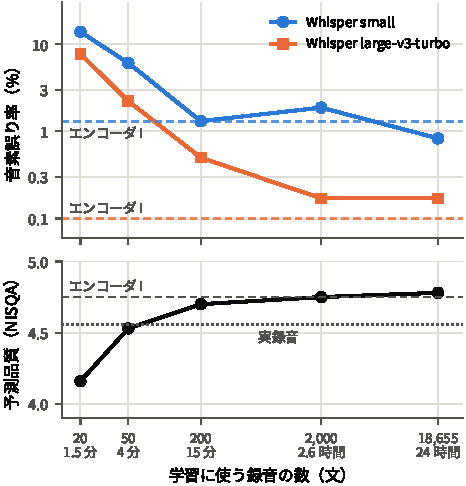
\includegraphics[width=\columnwidth]{fig_data_ja.pdf}
\caption{同じ音声合成モデルを、話者の録音を減らして学習した結果（テストの 100 文）。破線は
エンコーダ I が録音から作った合成音、点線は実録音。}
\label{fig:data}
\end{figure}

\textbf{録音を減らす}（図~\ref{fig:data}）。同じモデルを 200 文、つまり 15 分の音声で学習しても、
ほとんど誤りなく読まれる（0.5\%）。20 文、1 分半でも、large-v3-turbo は音素の 92\% を聞き取る。
ここまで小さいと、モデルはその言語の音をすべては聞いておらず、発音を誤る。それでも合成音の
予測品質は 4.16 あり、耳には、言葉を言い損なっている人に聞こえ、ぎりぎり聞き取れる。このうちどこまでが
潜在表現のおかげかは、\ref{sec:control} 節で調べる。

\textbf{代役はここでも効くか。}2,000 文の学習で、代役を通した誤差を外すと、その誤差が下げようと
するリスナー距離は 0.217 から 0.234 に上がる。しかし Whisper（0.3\% と 0.2\%）と音声記号の不一致
（27.2\% と 27.1\%）では、2 つのモデルの区別はつかない。手本の制御列は、それを書いたエンコーダが
「録音と同じに聞こえる」ように学習しているので、すでにそう聞こえる。エンコーダに不可欠だった
ものを、音声合成モデルは手本から受け継いでいる。

\textbf{100 話者}（表~\ref{tab:many}）。同じモデルを JVS の全体で学習した。100 話者（女性 51 人）で、
1 話者あたり約 100 文、12 分である（9,998 録音、20 時間）。モデルは話者ごとにベクトルを 1 つ持ち、
すべての音素とフレームに足す。声の高さは、話者ごとの平均と幅を基準に書く。声に伝えるのは、これまでと
同じく話者の性別と声の高さの中央値である。テストはエンコーダと同じで、8 話者が読む、どの話者の
学習にも出てこない 25 文である。テキストだけから書くと、large-v3-turbo の音素誤り率は 2.3\% で、
実録音（2.5\%）と並び、エンコーダの合成音（3.4\%）より低い。女性でも男性でも同じで、予測品質は
エンコーダと同じである。1 話者 20 文（各 2 分）では 3.4\%、5 文（各 35 秒）では 4.8\% になる。
音素の長さを話者のものにすると、ここでは悪くなる（4.4\%）。単一話者ではそうならなかった。原因は
調べていない。

\begin{table}[t]
\centering\footnotesize\setlength{\tabcolsep}{2.6pt}
\caption{JVS の 100 話者の音声合成。そのうち 8 話者が読む、どの話者の学習にも出てこない 25 文
（200 録音）。Whisper の誤り率（音素の \%）、音声記号の不一致（\%）、女性 4 人と男性 4 人の NISQA。}
\label{tab:many}
\begin{tabular}{@{}lrrrrr@{}}
\toprule
& small & large & 記号 & \multicolumn{2}{c}{NISQA 女 / 男}\\
\midrule
実録音 & 6.4 & 2.5 & -- & 4.80 & 4.87\\
別の実話者 & -- & -- & 32.1 & -- & --\\
エンコーダ I（録音から） & 8.2 & 3.4 & 29.3 & 3.91 & 4.25\\
TTS、長さは話者のもの & 8.5 & 4.4 & 34.1 & 3.87 & 4.37\\
TTS、テキストだけから & 7.0 & 2.3 & 34.2 & 3.89 & 4.39\\
\quad 1 話者 20 文で学習 & 8.7 & 3.4 & 39.0 & 3.70 & 4.31\\
\quad 1 話者 5 文で学習 & 9.7 & 4.8 & 42.2 & 3.52 & 4.30\\
\bottomrule
\end{tabular}
\end{table}

\textbf{誰の声か。}声に伝えているのは、話者の性別と声の高さの中央値である。人を聞き分ける
それ以外の手がかりは、制御列に入っていなければ失われる。話者照合モデル（x-vector のヘッドを持つ
WavLM~\cite{wavlm}）に 100 話者の中から最も近い話者を選ばせると、テストの実録音では 93.7\%、
エンコーダの合成音では 2.8\%、音声合成モデルの合成音では 2.4\% が当たる。性別は外さないので、
これは同性の約 50 人の中での偶然の水準である。現状のコーデックは、どの高さでも、性別ごとに
1 つの声である。

\textbf{話者ごとの体格。}CHIMERA の体格は連続である。成人男性から成人女性への軸と、大人から
子どもへの軸があり、声道の大きさと、そのうちの咽頭の割合を決める。この 2 つの値を、制御列は
そのままにして、100 話者それぞれに当てはめた。学習用の 6 文（最初の 4 秒）を候補の体格で鳴らし、
話者照合モデルが、その話者の録音に最も近いと判定する体格を残す。多言語のリスナーから見て録音
から離れるぶんは減点する。当てはめに使っていないテストの文で、照合モデルが本人を選ぶ割合は、
テストの 8 話者の中ではエンコーダの合成音で 26.5\% から 49.0\% に、100 話者の中では
2.8\% から 5.5\% に上がる。当てはめに使っていない別の照合モデル~\cite{unispeechsat}
でも同じで、8 話者の中で 24.0\% から 40.5\%、100 話者の中で 4.6\% から
8.2\% である。音声合成モデルの合成音も同じだけ上がる（8 話者の中で 28.0\% から
49.5\%）。ほかは動かない。large-v3-turbo の誤りは 3.4\% と 3.4\%、NISQA は
4.08 と 4.05 である。当てはまった声道の大きさは、男性のテンプレートを 1 として、女性で
平均 0.87（CHIMERA の女性の体格は 0.90）、男性で 0.98、ばらつきはどちらも 0.02 である。声門
（開放率、閉じ方の鋭さ、張り）まで当てはめると、別の照合モデルでは 8 話者の中で 51.5\% に
なるが、当てはめに使ったモデルでは体格だけと変わらない（48.0\%）。NISQA は 0.4 下がるが
（3.67）、試聴では悪くなったとは聞こえなかった。さらに進めた 3 つめの当てはめでは、体格の
4 つの値そのもの（男性のテンプレートより大きい声道も許す）、声門、そしてエンコーダが書かない
構えの癖 4 つ（声門の上の管をどれだけ狭く保つか、喉頭の高さ・口蓋帆・舌の根それぞれの一定の
ずれ）の、話者あたり 11 個の値を当てはめる。照合モデルが 8 話者の中から本人を選ぶ割合は
57.0\%（別のモデルで 59.5\%）、100 話者の中では 14.2\% と 12.2\% になる。
large-v3-turbo の誤りは 3.5\% のままで、NISQA は 3.88 である（男性は 4.35 で、
元の 4.25 より高い）。この一段で伸びたのは男性である。男性 49 人のうち 41 人で、声門の上の
管が範囲の半分以上狭められた（3\,kHz 付近の声の響きを作る）。女性では 51 人のうち
7 人である。男性のほとんどが同じ向きに動いたので、伸びの一部は、話者ごとの違いでは
なく、声全般が良くなったぶんである。話者ごとの値の代わりに、同性の平均の値を全員に与えると、
本人が選ばれる割合は 34.5\%（別のモデルで 29.0\%）である。平均の値はどの合成音も
同性のどの録音にも近づけ、聞き分けを生むのは話者ごとの値である。それでも、合成音は話者から遠い。話者の録音との類似度は 0.876 から
0.919 に上がるが、同じ話者の録音どうしは 0.98、同性の別の話者の録音とは 0.91 である。
合成音は、ようやく同性の別人と同じくらい本人に近い、というところである。

\textbf{女性と男性の違い。}照合を性別で分けると、当てはめの効き方が違う。100 話者の中では、
体格の 2 つの値は女性も男性も同じくらい押し上げる（本人と判定される割合が 2.4\% から 5.4\%、
3.3\% から 5.6\%）。11 個の値で伸びるのは男性である（20.5\%。女性は 8.2\%。別のモデルでは
17.4\% と 7.3\%）。テストの 8 話者の中では、女性 4 人は体格だけで 26\% から 73\% まで
聞き分けられ、男性は 25\% にとどまって、11 個の値で 40\% になる。試聴の判定も分かれた。男性は 11 個の値の合成音のほうが良い。女性は、声門を当てはめると
有声音がブザーのように聞こえる話者があり、どの合成音にも「華やかさ」が足りない。母音の強さを
帯域ごとに録音と比べると、これに対応するずれが見つかる。女性の母音は、1.6〜5.5\,kHz が録音より
7〜12\,dB 弱い。照合モデルに当てはめた声門は開放率が下がっていて、この帯域を 3〜5\,dB 戻す代わりに、
第 2 倍音を基本波に対して録音より 8.0\,dB 強くする（当てはめる前は 2.8\,dB）。男性の 11 個の値は、
1〜4\,kHz の不足を 9〜15\,dB から 4〜7\,dB に縮めていた。

低い倍音を変えずにこの帯域を戻す設定は、声門の閉じ方の鋭さである。これは照合モデルを使わずに
測れる。学習用の 6 文を鋭さを変えて鳴らし、有声の区間で 1.6〜5.5\,kHz の強さが録音と同じになる
値を取る。女性 51 人で 0〜0.62、平均 0.35 である（調整後の声は、いちばん柔らかい 0）。測った値で
鳴らすと、テストの女性の母音はこの帯域で録音から 3\,dB 以内になり、第 2 倍音のずれは 1.6\,dB に
なる。large-v3-turbo の誤りは変わらない（3.6\% と 3.7\%）。話者の聞き分けには効かない。
8 話者の中では、別の照合モデルが女性を本人と判定する割合が 58\% から 85\% に上がり、体格の
当てはめに使ったモデルでは 79\% から 68\% に下がるが、100 話者の中ではどちらのモデルでも
変わらない（7.8\% から 7.4\% と、7.8\% から 9.0\%）。鋭さは女性の合成音を全体として録音に
近づけるが、誰の声かは変えていない。代償もある。NISQA は 3.90 から 3.55 に下がり、5.5〜7.5\,kHz は録音より 7\,dB 強くなる（録音の母音は
この帯域で 10\,dB 落ち込むが、合成音は落ち込まない）。試聴では、鋭くすると足りなかった高域が出る。ただし測った値では、聞いた 2 人のうち 1 人にブザーの
ような響きが戻る。半分の値ではほとんど出ないので、女性の声には測った値の半分を採った（この帯域の
不足は 3.5〜6.4\,dB、NISQA は 3.68）。
鼻音にも同じ向きのずれがある。女性の鼻音は、母音に対して録音より 4.8\,dB 弱く、第 2 倍音が
10\,dB 強い。シミュレータの鼻腔に付く副鼻腔を 14\,cm$^3$ から 24\,cm$^3$ にすると第 2 倍音のずれは
5\,dB に縮むが、試聴では聞き分けられなかった。

\section{潜在表現のおかげか: 対照実験}\label{sec:control}
\ref{sec:tts} 節のモデルは、少ないデータで学習でき、崩れ方が穏やかである。そのうちどこまでが
制御列のおかげかを見るために、同じモデルに、ニューラルネットが音に戻す潜在表現を書かせた。
\begin{itemize}
\item \textbf{メルスペクトログラム}（100 帯域、毎秒 93.75 フレーム）。UnivNet ボコーダ~\cite{univnet}
で音にする。この形のモデルの本来の出力先である~\cite{fastspeech2}。
\item \textbf{EnCodec} の量子化前の潜在表現~\cite{encodec}（128 次元、毎秒 75 フレーム）。
\item \textbf{Mimi} の潜在表現~\cite{moshi}。デコーダが受け取る形、つまり 32 個のコードブックが表す
ベクトルである（512 次元、毎秒 12.5 フレーム）。
\end{itemize}
3 つとも公開されているモデルで、24\,kHz でそのまま使う。テキストの入力、音素の長さ、層、学習の
スケジュール、残す重みの選び方は \ref{sec:tts} 節と同じである。フレームの層は毎秒 100 フレームで
動かし、その出力を潜在表現のフレームレートまで平均する。対照のモデルには FastSpeech\,2 のピッチ
予測器を付けた（これらの潜在表現にはピッチのチャネルがないため）。物理モデルは、ここでは代役を
通した誤差を外して学習した。これで 4 つのモデルの誤差は同じになる。録音の潜在表現との差
（各値をその広がりで割ったもの）と、音素の長さの誤差である。

\begin{figure}[t]
\centering
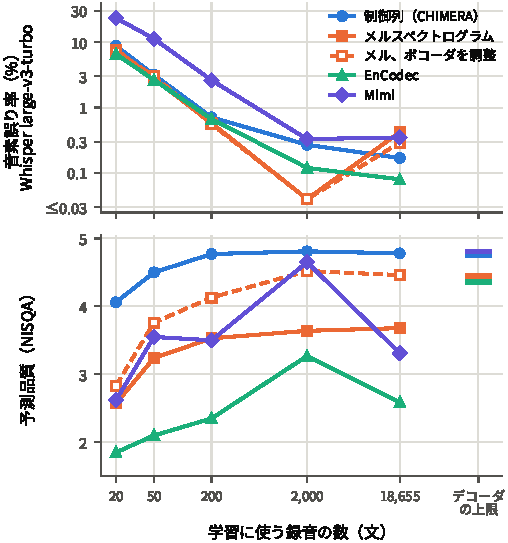
\includegraphics[width=\columnwidth]{fig_control_ja.pdf}
\caption{同じモデルに 4 種類の潜在表現を書かせた結果（テストの 100 文）。上: Whisper の読み誤り。
下: 予測品質。右端の横棒は各デコーダの上限（録音を潜在表現にして戻した音。制御列ではエンコーダ I の
合成音）。破線は、モデルが書いたスペクトログラムでボコーダを調整したもの。}
\label{fig:control}
\end{figure}

\begin{table}[t]
\centering\footnotesize\setlength{\tabcolsep}{3pt}
\caption{対照実験（テストの 100 文）。列は学習に使った録音の数。上限は図~\ref{fig:control} と同じく
デコーダのもの（調整したボコーダでは、全データで調整したものに実際のスペクトログラムを与えた音）。
「交差」は、各録音のスペクトログラムを、その録音を学習していないモデルに書かせて調整したもの。
$^\dagger$\ref{sec:tts} 節のモデル（代役を通した誤差あり）。}
\label{tab:control}
\begin{tabular}{@{}lrrrrrr@{}}
\toprule
& 20 & 50 & 200 & 2,000 & 18,655 & 上限\\
\midrule
\multicolumn{7}{@{}l}{\emph{Whisper large-v3-turbo の音素誤り率（\%）}}\\
制御列 & 8.8 & 3.2 & 0.7 & 0.3 & 0.2$^\dagger$ & 0.1\\
メルスペクトログラム & 7.7 & 2.8 & 0.6 & 0.0 & 0.4 & 0.1\\
\quad ボコーダを調整 & 7.2 & 3.0 & 0.6 & 0.0 & 0.3 & 0.1\\
\quad 同、交差 & 8.2 & 3.4 & 0.8 & 0.0 & -- & --\\
EnCodec & 6.6 & 2.6 & 0.7 & 0.1 & 0.1 & 0.1\\
Mimi & 23.4 & 11.2 & 2.6 & 0.3 & 0.3 & 0.1\\
\multicolumn{7}{@{}l}{\emph{NISQA}}\\
制御列 & 4.06 & 4.50 & 4.77 & 4.81 & 4.78$^\dagger$ & 4.75\\
メルスペクトログラム & 2.57 & 3.24 & 3.53 & 3.64 & 3.68 & 4.45\\
\quad ボコーダを調整 & 2.83 & 3.76 & 4.13 & 4.52 & 4.46 & 4.62\\
\quad 同、交差 & 3.18 & 3.64 & 3.92 & 4.30 & -- & --\\
EnCodec & 1.85 & 2.10 & 2.35 & 3.27 & 2.59 & 4.36\\
Mimi & 2.62 & 3.55 & 3.50 & 4.65 & 3.31 & 4.81\\
\bottomrule
\end{tabular}
\end{table}

\textbf{言葉は、どの潜在表現でも少ないデータで足りる。}テストの文では、メルスペクトログラムと
EnCodec は、どのデータ量でも制御列と同じだけ聞き取れる（図~\ref{fig:control}、表~\ref{tab:control}）。
音素の誤りは、200 文で 0.6\%、0.7\%、0.7\%、20 文で 7.7\%、6.6\%、8.8\% である。もっとデータが要るのは、
次元が大きくフレームの粗い Mimi だけである。つまり、\ref{sec:tts} 節の「少ないデータで足りる」は
モデルの性質（音素とアクセントを入力し、音素の長さを与え、自己回帰をしない）であり、制御列の
性質ではない。制御列がメルスペクトログラムより予測しやすいわけでもない。学習に使っていない文での
モデルの誤差は、値の広がりに対する割合で見ると両者で同じで（2,000 文で 0.17）、2 つのコーデックでは
ずっと大きい（0.46 と 0.47）。

\textbf{違うのは音である。}シミュレータの合成音は、どのデータ量でも予測品質が 4.1〜4.8 ある。
デコーダをそのまま使うと、メルスペクトログラムは 2.6〜3.7 で、そのボコーダは実際のスペクトログラムなら 4.45 を出す。EnCodec は
1.9〜3.3（上限 4.36）、Mimi は 2.6〜4.7（上限 4.81）である。相対的に同じ大きさの誤差が、ボコーダでは 1 点の低下になり、シミュレータ
では何も起こさない。ぼやけたスペクトログラムは声のスペクトログラムではないが、ぼやけた調音は調音の
ままである。データを増やすだけでは
差は埋まらない。18,655 文すべてで学習しても、合成音はメルスペクトログラムで 3.68、EnCodec で 2.59、
Mimi で 3.31 である（どれもほぼ誤りなく聞き取れる）。また、コーデックの品質はデータ量に対して
単調ではない。2,000 文では Mimi が 4.65、EnCodec が 3.27 で、どちらも全データのときより高い。
覚え込めなくなったモデルは平均を取る。モデルの予測は、フレーム間の動きを、制御列では 0.95、
メルスペクトログラムでは 0.78 保つ。EnCodec では 2,000 文で 0.61、全データで 0.49 である。制御列には、
回帰が失う種類の細部がほとんどない。（どのセルも学習 1 回の結果で、コーデックの上下のうちどこまでが
偶然かは分からない。）

\textbf{モデルが書いたスペクトログラムでボコーダを調整する。}ボコーダは、実録音の
スペクトログラムで学習されている。モデルが書くスペクトログラムの音を良くする普通の方法は、
それでボコーダを調整することである~\cite{tacotron2,hifigan}。入力は、モデルが学習に使った録音に
ついて、その録音の音素の長さとピッチを与えて書かせたスペクトログラム、目標は録音の音である。
これを、各データ量で、その録音だけを使って行った。UnivNet を、学習されたときと同じ誤差と、同じ
識別器で学習し続ける（識別器は作者の公開チェックポイントに入っている）。1 ステップに 0.68 秒の
区間を 16 個、データ量に応じて 1,500〜15,000 ステップである。識別器は欠かせない。スペクトルの
誤差だけで調整すると、検証の文の合成音は 3.6 から 2.7 に下がり、新しく作って 10,000 ステップ
学習した識別器では 1.4 に下がった。残すボコーダは、検証の文で NISQA が最も高いものである。
NISQA で選んでいるのはここだけで、対照に有利な選び方である（最後のステップのボコーダなら、
200 文と 2,000 文で 4.02 と 4.36 になる。全データでは、最後のステップが残った）。

調整すると、メルスペクトログラムの合成音はどのデータ量でも良くなる（表~\ref{tab:control}、
図~\ref{fig:control} の破線）。20 文で 2.57 から 2.83、200 文で 3.53 から 4.13、2,000 文で 3.64 から
4.52、全データで 3.68 から 4.46 である。Whisper の読み誤りは変わらない。2,000 文以上では、調整後の
合成音は実録音（4.56）にほぼ並ぶ。調整したボコーダが実際のスペクトログラムから出す音（4.62）
よりは少し低い。
話者の音声が 2 時間半あれば、この方法は効く。少ないと効きが小さい。データが少ない場合のために、
各録音のスペクトログラムを、その録音を学習していないモデルに書かせる変種（5 分割）も試した。
ボコーダが、新しい文と同じだけぼやけたスペクトログラムで学習できる。20 文では効くが（3.18）、
それより多いと効かない（50 文、200 文、2,000 文で 3.64、3.92、4.30）。良いほうを取っても、制御列の
合成音との差は 20 文で 0.9、50 文で 0.7、200 文（15 分）で 0.6 ある。2,000 文と全データでは
0.3 で、その大半は、シミュレータの音が実録音そのものより高く付くぶんである。

\textbf{コーパスと違う文。}コーパスにない 12 文（\ref{sec:tts} 節）では、対照はテストの文より多く
崩れる。200 文で学習したとき、large-v3-turbo の誤り率はメルスペクトログラム 4.0\%、EnCodec 3.0\% に
対し、制御列は 0.4\% である。12 文なので区間は広い（[0.8, 9.2]、[0.2, 7.5]、[0.0, 1.0]）。ボコーダを調整すると、
メルスペクトログラムは 1.4\%（[0.6, 2.2]） になる。

\textbf{この対照から言えないこと。}ニューラルデコーダは話者の声を返す。その上限は話者自身の声で
ある。シミュレータの声はシミュレータのものである（\ref{sec:tts} 節）。また、ニューラルデコーダには
シミュレータの鋭い破裂の音がない（1 秒に 0.1〜0.3 回、発話より 25\,dB 小さく、実録音と同じ。
シミュレータは 0.5〜0.6 回で 16\,dB）。調整したのはメルスペクトログラムのデコーダだけである。回帰の代わりに潜在表現の生成モデルを
使うという、もう 1 つの普通の方法は試していない。そして、品質は 1 つの予測モデルの値である。
NISQA には合成音声の自然さを予測するモデルもあり、そちらでは順位が逆になる。シミュレータの
合成音はどのデータ量でも 2.7〜2.9、メルスペクトログラムは 3.5〜3.9（ボコーダを調整すると
3.6〜4.2）、実録音は 4.5 である。低く付けられているのはモデルではなく声である（エンコーダ I が
録音から作った合成音も 2.7）。試聴と合っていたのは、品質のスコアのほうである（\ref{sec:voice} 節と、
この節の調整していないデコーダの合成音）。ボコーダの調整で上がる 0.5 ほどの差は、試聴では
はっきりしなかった。

\section{公開に向けて}\label{sec:release}

ここまでのモデルは、どれも公開できない。エンコーダ I は mHuBERT を通して録音を聞き、mHuBERT を
物差しにして学習している。その重みの一部はエンコーダの重みの中にあり、ライセンスは非営利に
限られる（CC BY-NC-SA 4.0）。JVS は研究用で再配布できず、Hi-Fi-CAPTAIN も CC BY-NC-SA である。
この節では、公開できる材料だけで作り直す。TSP（BSD ライセンス）、Emilia-YODAS~\cite{emilia}
（Creative Commons ライセンスの動画から切り出した音声、CC BY 4.0）、重みが Apache-2.0 か MIT の
モデル（wav2vec 2.0 base、XLS-R~\cite{xlsr}、日本語で学習した HuBERT~\cite{jtube}）である。

\textbf{2 つの基準の声。}話者ごとに当てはめた設定は、その話者の録音がないと作れない。テキスト
音声合成のデモには録音がないので、決まった設定を 2 つの声にまとめた。高い声は、
\ref{sec:voice} 節の調整後の声に、女性の体格の平均、大きい副鼻腔、試聴で選んだ閉じ方の鋭さの
平均（0.18）を足したものである。低い声は、シミュレータの成人男性に 2 つの構えを足したもので
ある（喉頭の上の狭め 0.78 と、舌の根を 0.35\,cm 前へ）。男性の 11 個の値を 1 つずつ試すと、
合成音を照合モデルにとって本人に近づけるのはこの 2 つだった（テストの男性で 0.870 から 0.903。
11 個すべての平均では 0.899）。どちらの声を使うかは、声の高さではなく性別で決める。JVS には声の
高さの中央値が 196\,Hz の男性がいて、TSP の女性は 173\,Hz から始まる。体格を声の高さで混ぜると、
男性の合成音は本人から遠ざかった（0.850 から 0.812）。エンコーダの学習に使ってきた声も、
弱い形で同じことをしていた。150\,Hz を超える男性に、高い声用の柔らかい声源を混ぜていた
のである。テストの男性 4 人のうち 3 人がこれにあたり、第 2 倍音が 5.6\,dB 弱かった。
エンコーダ I の制御列を 2 つの声で鳴らすと、女性は話者ごとの設定の平均とほぼ同じになり、男性は
11 個の値とほぼ同じところまで来る（1〜4\,kHz の不足は 5〜8\,dB、第 2 倍音のずれは 1.1\,dB、
類似度は 0.900 と 0.917）。誰の声かは区別できないが、それはこの声の役目ではない。

この 2 つの声には、つまみがある。明るさを 1 目盛り上げると、閉じ方の鋭さが 0.18、低い声では
喉頭の上の狭めも 0.22 増える。母音の 2.5〜4\,kHz は 1 目盛りで 3〜5\,dB 動き、第 2 倍音は
1\,dB も動かない。また、制御列は体格にあまり依存しない。女性の制御列を低い声で 10 半音下げて
鳴らしても、男性の制御列を高い声で 9 半音上げて鳴らしても、前と同じくらい読める
（large-v3-turbo の誤りは 3.1〜3.8\%）。この入れ替えから、女性の点が低い理由も分かる。男性の
制御列は、高い声で鳴らすと女性と同じ点になる（音声記号の不一致が 25.8\% から 31.7\%、NISQA が
4.34 から 3.59）。女性の制御列は、低い声で鳴らすと男性と同じ点になる（31.7\% から 29.3\%、
3.64 から 4.74）。原因は高い声そのもので、女性のために書かれた制御列ではない。

\begin{table}[t]
\centering\footnotesize\setlength{\tabcolsep}{2.1pt}
\caption{公開に向けたエンコーダ。表~\ref{tab:japanese} と同じテストでの、Whisper large-v3-turbo の
誤り（\%）と音声記号の不一致（\%）。1 行目以外は 2 つの基準の声で鳴らす。各行は、上の行から
1 つだけ替えたもの（J0 は物差しと入口のモデル、J は JVS の録音、J2 は物差し）。公開できる材料
だけで学習したのは J と J2 である。}
\label{tab:release}
\begin{tabular}{@{}lrrrrrr@{}}
\toprule
& \multicolumn{2}{c}{JVS} & \multicolumn{2}{c}{HFC+JSUT} & \multicolumn{2}{c}{TSP（英語）}\\
& 誤り & 記号 & 誤り & 記号 & 誤り & 記号\\
\midrule
I（これまでの声） & 3.4 & 29.3 & 0.4 & 27.3 & 3.2 & 9.4\\
I を基準の声で & 3.4 & 28.8 & 0.5 & 27.6 & 4.2 & 9.7\\
I$'$（基準の声で学習） & 3.6 & 28.0 & 0.5 & 27.2 & 4.1 & 10.1\\
J0（+ XLS-R） & 5.0 & 32.8 & 1.6 & 31.6 & 7.0 & 12.7\\
J（+ Emilia-YODAS） & 4.9 & 31.5 & 1.2 & 30.7 & 5.0 & 10.6\\
J2（物差しを日本語の HuBERT に） & 3.6 & 28.1 & 0.5 & 27.5 & 4.6 & 10.5\\
\bottomrule
\end{tabular}
\end{table}

\textbf{エンコーダ。}\ref{sec:encoder} 節と同じ方法で比べると、XLS-R の第 16 層は、日本語の合成音を
「別の話者より録音から遠い」と聞く。mHuBERT の第 8 層と同じである（$d'$ は 0.97 と 1.32）。英語の
合成音でもそう聞く（0.33 と $-0.05$）。これを物差しにし、入口は wav2vec 2.0 base にした。
Emilia-YODAS には話者の性別が書かれていないが、声を選ぶには性別が要る。声の高さで迷いのない
話者（中央値が 135\,Hz 未満か 235\,Hz 超）はそれで決め、その間の話者は、照合モデルのベクトルが
男女どちらの平均に近いかで決めた。JVS と TSP の同じ範囲の話者では、90〜95\% が合う。何を替えると
どれだけ損をするかは、3 つのエンコーダで分けた（表~\ref{tab:release}）。2 つの声を通して
学習し直す効果は小さい（I$'$）。JVS の音声記号の不一致は 28.8\% から 28.0\% になり、英語は少し
悪くなる。大きいのは、使えるモデルに替える損である。mHuBERT を XLS-R と wav2vec 2.0 base に
替えると（J0）、JVS の不一致は 32.8\%、Whisper の誤りは 3.6\% から 5.0\% になる。録音を替える
損はない。JVS を Emilia-YODAS に替えると（J。各言語 300 話者、6 文ずつ、約 6 時間）、どのテストも
良くなる。J は JVS の録音を一度も聞いていないが、JVS のテストでも良くなる。話者は 86 人から
600 人に増えている。差し引きで、J は I$'$ より日本語の音声記号の不一致で 3.5 ポイント、Whisper の
誤りで約 1 ポイント悪い。英語の差は 0.5 ポイント以内で、NISQA は変わらない。
この損は物差しのもので、物差しを替えると消える。J0 と同じ録音でさらに 3 つのエンコーダを学習すると、
日本語だけで学習した HuBERT（hubert-base-jtube~\cite{jtube}、MIT、第 8 層）を物差しにしたものは、
音声記号の不一致が J0 より 1.8 ポイント小さく、Whisper の誤りは日本語でも英語でも I$'$ の水準に
戻る（JVS で 3.3\%、TSP で 5.3\%。入口を XLS-R にする、あるいは物差しを XLS-R の第 12 層に
すると、その半分ほど戻る）。この物差しと Emilia-YODAS を組み合わせた J2 は、公開できる材料だけで
学習して、どのテストでも I$'$ と並ぶ。

\textbf{テキスト音声合成。}\ref{sec:tts} 節のモデルを、公開できる録音だけで学習し直した。録音は 2 種類、
モデルの作りも 2 種類である。Emilia-YODAS の日本語は話し言葉で、言葉は認識器が書き起こして
おり、話者はほとんどが男性である（約 800 人のうち、女性と推定されたのは 100 人ほど）。
Common Voice~\cite{commonvoice} はボランティアによる文の読み上げ（CC0）で、女性と男性が同数
いるが、部屋もマイクも人それぞれである。モデルは、これまでのように話者ごとにベクトルを持つか、
その代わりに話者の 2 つの数（高い声の割合と、話す速さ）を入力にする。後者では、誰も録音して
いない声は、つまみの位置になる。分かったことは 3 つある（誤りは Whisper large-v3-turbo による
もので、JVS のテスト文を録音と同じ速さで読ませた値）。1 つ目。モデルは、エンコーダがその録音を
どれだけ写せたかを引き継ぐ。J の制御列で鳴らすと、Common Voice の録音は音素の 13.9\%、
Emilia-YODAS は 7.7\% が誤って読まれる（録音そのものは 3.2\% と 4.0\%）。その制御列で学習した
Common Voice のモデルは、どの話者の声で読ませるかによって 6.6〜15.7\% を誤る。J2 の制御列では
7.0\% と 5.0\% になる。2 つ目。声を入力にしたモデルは、話者ベクトルのモデルより良く読む。同じ
制御列で、低い声が 5.4\%、高い声が 4.1\%（話者ベクトルでは 11.7\% と 5.7\%）である。十数文から
学習したベクトルは、その録音の悪さも覚えてしまう。3 つ目。J2 の制御列では、つまみ用のモデルが
実録音に並ぶ。低い声は Emilia-YODAS で学習したものが 2.4\%、高い声は Common Voice で学習した
ものが 2.8\% で、実録音は 2.5\%、JVS で学習したモデルは 2.3\% である。きれいな例の多い側の声が、
そのコーパスで良くなる。途中で直したことが 2 つある。話し言葉は読み上げより 3 割速いので、
速さは指定するようにした。また、音素の対応付けは、スタジオの読み上げでは 12 エポックで学習
できたが、どちらのコーパスでも 40 エポックが要る。これらのモデルの試聴はまだである。

\textbf{ブラウザの中で。}エンジンは、制御列の再生部と合わせて WebAssembly になり（651\,kB）、
Python のモジュールと同じサンプルを、1 コアで実時間の 5 倍以上の速さで出す。ページはサーバから
文の制御列（数キロバイトの数値）だけを受け取り、音を自分で作る。声の高さと明るさは、話して
いる途中でも変えられる。

\section{考察}\label{sec:discussion}
\textbf{効いたこと。}\emph{声を通して教える。}制御列を真似ると、同じことの言い方の平均を取って
しまう。シミュレータの粗いモデルを通して「その制御列が正しく聞こえるか」を教えると、エンコーダの
単語誤り率は 19.5\% から 6.5\% に下がり、探索は要らなくなった。
\emph{何を学ぶかはリスナーが決める。}英語のリスナーは日本語の誤りを聞き分けず、それとの距離が
下がり続けても、物差しは動かなかった。
\emph{計測が見落としたものを、試聴が見つけた。}\ref{sec:voice} 節の音はどれも、まず耳で聞かれ、
耳で場所が特定され、そのあとで計測された。計測は 2 度、違う場所を見ていた。また、品質の予測
モデルだけに合わせると、抜け道を見つけた。
\emph{言葉は少ないデータで足りる。デコーダが効くのは音である。}素朴な非自己回帰モデルは、
与えたデータの 100 分の 1 で聞き取れるようになり、100 話者を 1 人 35 秒から学習する。対照実験に
よれば、これは制御列の手柄ではない。メルスペクトログラムも同じ速さで学習される。物理デコーダが
加えるのは、少ししか学習していないモデルの音がきれいな音声のままであることである。ニューラル
ボコーダも、モデルの出力で調整すればそこに届くが、それには話者の音声が何時間も要る。数分では
届かない。

\textbf{限界。}このコーデックが運ぶのは、言葉とそのタイミングと声の高さであり、誰が話しているかは
わずかしか運ばない。声に伝えるのが話者の性別と声の高さの中央値だけだと、話者照合モデルは同性の
話者を聞き分けられない。体格・声門・構えを話者ごとに当てはめても、本人を選べるのは 8 話者の中で
57.0\%、100 話者の中では 14.2\% である（\ref{sec:tts} 節）。音色はシミュレータのもののままである。
女性の声は、母音の 1.6〜5.5\,kHz が録音より弱く、試聴でも男性の声より現実味に欠ける。
破裂音の音は話者より鋭く、音声合成モデルの合成音ではさらに多い（1 秒に 0.61 回で発話より
15.4\,dB 小さい。エンコーダは 0.54 回と 16.3\,dB、実録音は 0.27 回と 25.8\,dB）。日本語の「え」の
音色はまだ外れている。点数は ASR と 1 つの品質予測モデルによるもので、各モデルの学習は 1 回ずつ、
試聴は 1 人である。対照実験で調整したのは、メルスペクトログラムのデコーダだけである。EnCodec と Mimi の
デコーダはそのまま使い、回帰の代わりに潜在表現の生成モデルを使うことは試していない。また、
NISQA の自然さのモデルは、シミュレータの声をニューラルデコーダの合成音より低く付ける
（\ref{sec:control} 節）。
アクセントは Open JTalk の推定によるので、推定が外れたところでは外れる。

\section{おわりに}
声の物理モデルは、微分可能でなくても、改造しなくても、音声コーデックのデコーダになる。学習した
代役を通して教えたエンコーダは、録音からその制御列を 1 回の推論で書き、合成音は実録音に近い
水準で聞き取れる。この潜在表現の誤りは、滑舌の悪さとして現れる。シミュレータ由来の音を仕組みまで
たどって設定で取り除けたのは、そのどの部分にも意味があるからである。そして、この潜在表現は
テキストから書ける。小さなモデルがエンコーダと並び、1 話者の 15 分の音声で聞き取れるように
なり、100 話者では見たことのない文を実録音と同じだけ聞き取れる音で読む。少ないデータで足りる
のはモデルの性質である（メルスペクトログラムと 2 つのニューラルコーデックを使った対照実験が
そう示す）。物理デコーダの性質は、データが数分しかなくても、その結果がきれいな音声であること
である。ニューラルボコーダは、モデルの出力で調整しても、同じところに届くのに何時間もの音声を
要する。

\section*{謝辞}
CHIMERA を公開している Jameson Hodge 氏、および TSP speech database、JVS、JSUT、Hi-Fi-CAPTAIN、
wav2vec\,2.0、mHuBERT-147、Whisper、NISQA、Open JTalk の作者の方々に感謝する。

\begin{thebibliography}{99}\footnotesize
\setlength{\itemsep}{0pt}
\bibitem{encodec} A.~Défossez, J.~Copet, G.~Synnaeve, Y.~Adi. High fidelity neural audio
compression. \emph{TMLR}, 2023.
\bibitem{moshi} A.~Défossez et al. Moshi: a speech-text foundation model for real-time dialogue.
arXiv:2410.00037, 2024.
\bibitem{pocketja} Claude, T.~Mori. Pocket TTS learns Japanese: Training data and distillation for
a drop-in 100M-parameter model. Technical report, 2026.
\bibitem{sparc} C.~J.~Cho, P.~Wu, T.~S.~Prabhune, D.~Agarwal, G.~K.~Anumanchipalli. Coding speech
through vocal tract kinematics. arXiv:2406.12998, 2024.
\bibitem{arti6} J.~Lee et al. ARTI-6: Towards six-dimensional articulatory speech encoding.
arXiv:2509.21447, 2025.
\bibitem{difftlm} E.~M.~Chen, J.~W.~Lee, V.~Sitzmann. Reconstructing the vocal tract with
differentiable acoustic simulation. arXiv:2609.36737, 2026.
\bibitem{vtl} P.~Birkholz. VocalTractLab. \url{https://www.vocaltractlab.de}.
\bibitem{chimera} J.~Hodge. CHIMERA: a physical-modeling voice synthesizer.
\url{https://github.com/jamesondh/chimera-vocal-synth}, 2026.
\bibitem{tsp} P.~Kabal. TSP speech database. Technical report, McGill University, 2002.
\bibitem{jvs} S.~Takamichi et al. JVS corpus: free Japanese multi-speaker voice corpus.
arXiv:1908.06248, 2019.
\bibitem{hificaptain} NICT. Hi-Fi-CAPTAIN corpus.
\url{https://ast-astrec.nict.go.jp/en/release/hi-fi-captain/}.
\bibitem{jsut} R.~Sonobe, S.~Takamichi, H.~Saruwatari. JSUT corpus: free large-scale Japanese
speech corpus for end-to-end speech synthesis. arXiv:1711.00354, 2017.
\bibitem{whisper} A.~Radford et al. Robust speech recognition via large-scale weak supervision.
\emph{ICML}, 2023.
\bibitem{openjtalk} Open JTalk. \url{https://open-jtalk.sourceforge.net}.
\bibitem{xlsrphone} Q.~Xu, A.~Baevski, M.~Auli. Simple and effective zero-shot cross-lingual
phoneme recognition. \emph{Interspeech}, 2022.
\bibitem{nisqa} G.~Mittag, B.~Naderi, A.~Chehadi, S.~Möller. NISQA: A deep CNN-self-attention
model for multidimensional speech quality prediction with crowdsourced datasets.
\emph{Interspeech}, 2021.
\bibitem{praat} P.~Boersma. Accurate short-term analysis of the fundamental frequency and the
harmonics-to-noise ratio of a sampled sound. \emph{IFA Proceedings} 17, 1993.
\bibitem{distal} M.~I.~Jordan, D.~E.~Rumelhart. Forward models: Supervised learning with a distal
teacher. \emph{Cognitive Science} 16(3), 1992.
\bibitem{wav2vec2} A.~Baevski, Y.~Zhou, A.~Mohamed, M.~Auli. wav2vec 2.0: A framework for
self-supervised learning of speech representations. \emph{NeurIPS}, 2020.
\bibitem{mhubert} M.~Zanon~Boito, V.~Iyer, N.~Lagos, L.~Besacier, I.~Calapodescu. mHuBERT-147: A
compact multilingual HuBERT model. \emph{Interspeech}, 2024.
\bibitem{univnet} W.~Jang, D.~Lim, J.~Yoon, B.~Kim, J.~Kim. UnivNet: A neural vocoder with
multi-resolution spectrogram discriminators for high-fidelity waveform generation.
\emph{Interspeech}, 2021.
\bibitem{tacotron2} J.~Shen et al. Natural TTS synthesis by conditioning WaveNet on mel
spectrogram predictions. \emph{ICASSP}, 2018.
\bibitem{hifigan} J.~Kong, J.~Kim, J.~Bae. HiFi-GAN: Generative adversarial networks for
efficient and high fidelity speech synthesis. \emph{NeurIPS}, 2020.
\bibitem{unispeechsat} S.~Chen et al. UniSpeech-SAT: Universal speech representation learning
with speaker aware pre-training. \emph{ICASSP}, 2022.
\bibitem{wavlm} S.~Chen et al. WavLM: Large-scale self-supervised pre-training for full stack
speech processing. \emph{IEEE JSTSP} 16(6), 2022.
\bibitem{fastspeech2} Y.~Ren et al. FastSpeech 2: Fast and high-quality end-to-end text to speech.
\emph{ICLR}, 2021.
\bibitem{ota} R.~Badlani, A.~Łańcucki, K.~J.~Shih, R.~Valle, W.~Ping, B.~Catanzaro. One TTS
alignment to rule them all. \emph{ICASSP}, 2022.
\bibitem{emilia} H.~He et al. Emilia: A large-scale, extensive, multilingual, and diverse dataset
for speech generation. arXiv:2501.15907, 2025.
\bibitem{xlsr} A.~Babu et al. XLS-R: Self-supervised cross-lingual speech representation learning
at scale. Interspeech, 2022.
\bibitem{jtube} sarulab-speech. hubert-base-jtube: a HuBERT model trained on JTubeSpeech.
\url{https://huggingface.co/sarulab-speech/hubert-base-jtube}.
\bibitem{commonvoice} R.~Ardila et al. Common Voice: A massively-multilingual speech corpus. LREC, 2020.
\end{thebibliography}
\end{document}
